\documentclass[12pt]{beamer}
\usepackage[utf8]{inputenc}
\usepackage{caption}
\usepackage{subcaption}
\usetheme{Berkeley}
\usecolortheme{beaver}

\title{Decision Trees}
\author[Pattanin (Mill) Luangamornlert]{Pattanin (Mill) Luangamornlert\\[1ex]  {\small Supervised by Louis Aslett and Peter Craig}}
\institute{Durham University}


\begin{document}

\frame{\titlepage}

\begin{frame}{Introduction}
   Decision Trees are a form of non-parametric statistics as well as machine learning. They show decision paths from a parent node to a child node to predict the likely outcome of an event given certain inputs.
   \begin{figure}
       \centering
       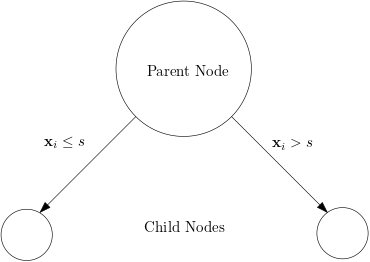
\includegraphics[width = 5cm]{ipefile/simpledecisionsplit.png}
       \caption{A generic decision tree diagram}
       \label{fig:basicdt}
   \end{figure}
\end{frame}



\begin{frame}{CART}
\begin{itemize}
    \item CART \cite{BreimanDT} was put together by Leo Breiman, Jerome Friedman, Richard Olshen, and Charles Stone in 1984 in their book, Classification and Regression Trees.
    
    \item It is the most popular method of Decision Trees today and is the basis for most modern tree based machine learning methods.
\end{itemize}
\end{frame}

\begin{frame}{Example Tree}
    Here is an example of a Classification Tree using CART using the Penguins Dataset \cite{penguins}:
    \begin{figure}
        \centering
        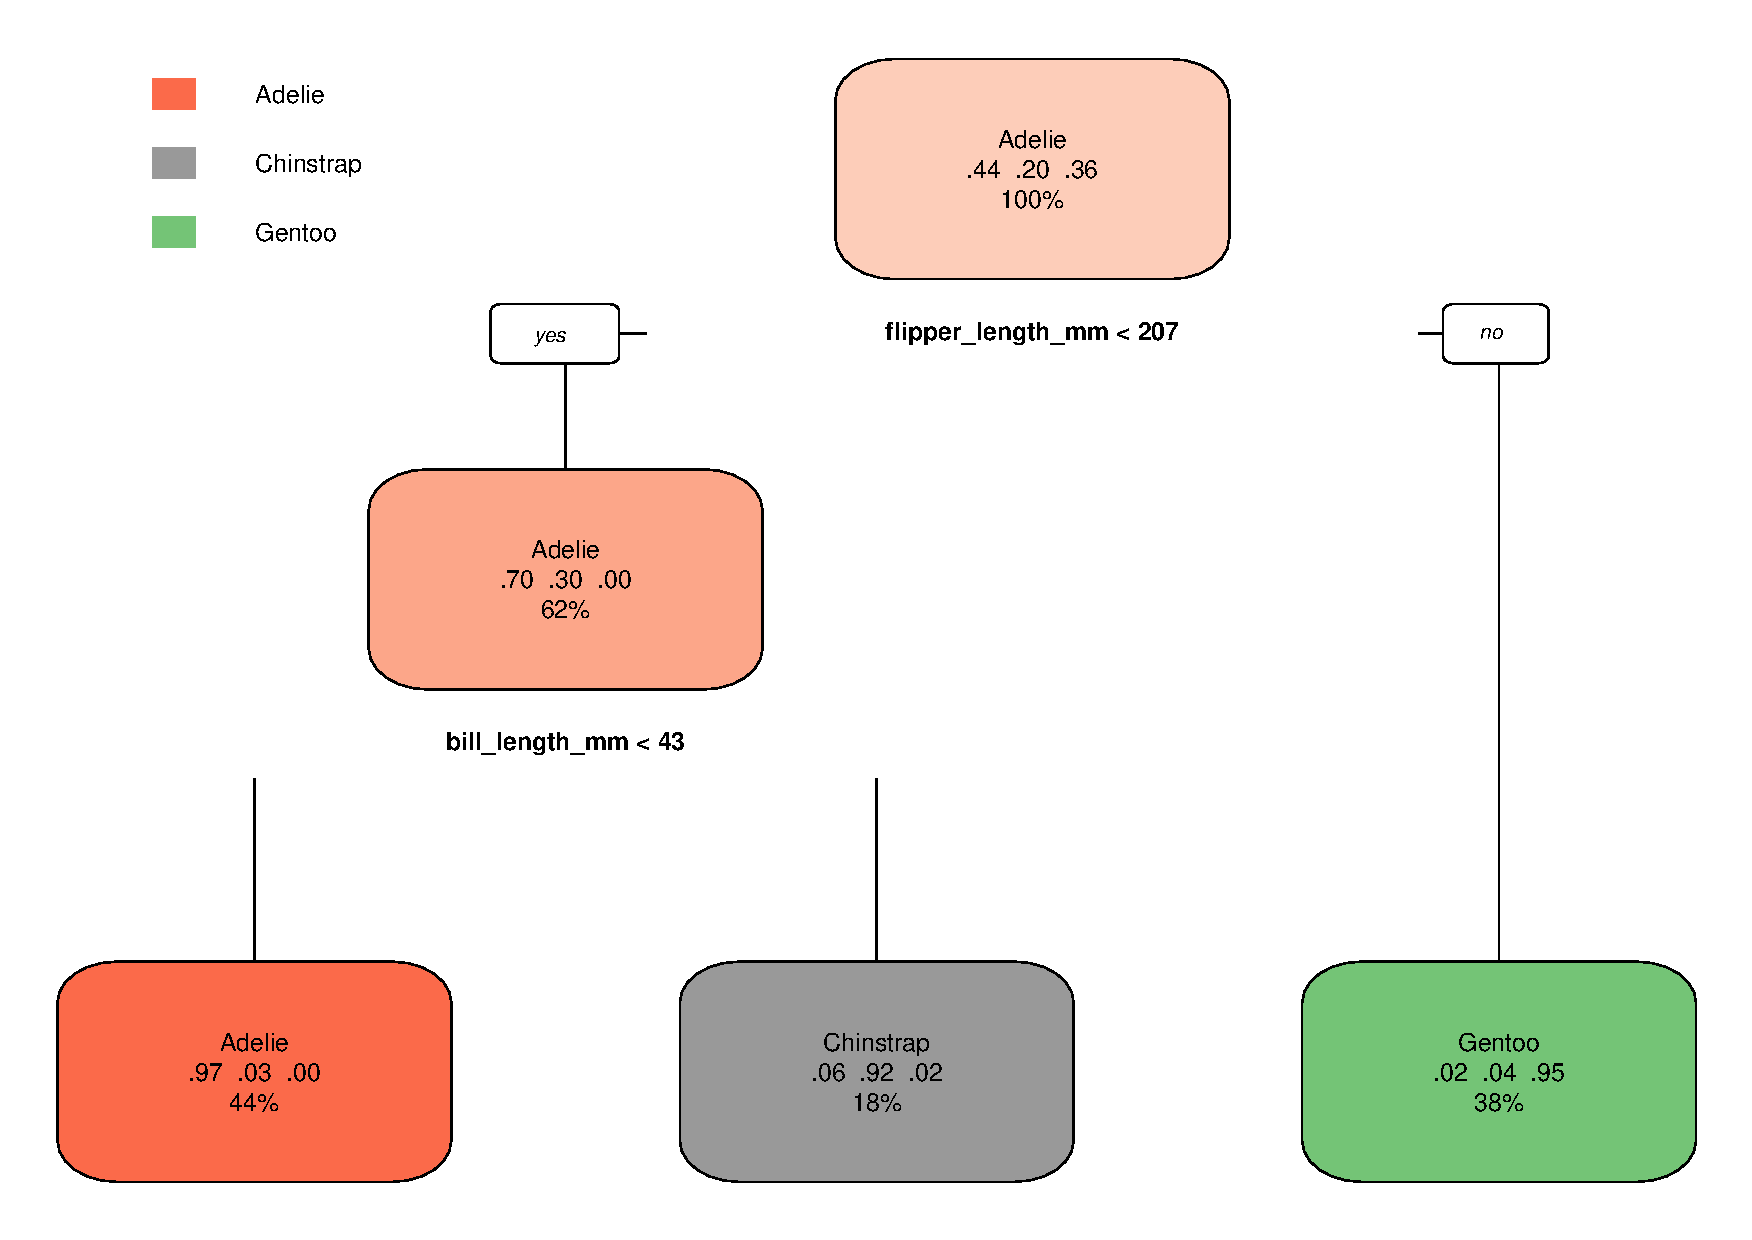
\includegraphics[width = 7cm]{presentation/Penguintree.pdf}
        \caption{Classification Tree for Penguins data}
        \label{fig:pentree}
    \end{figure}
\end{frame}

\begin{frame}{Visual Representation of Penguin Tree}
    \begin{figure}
        \centering
        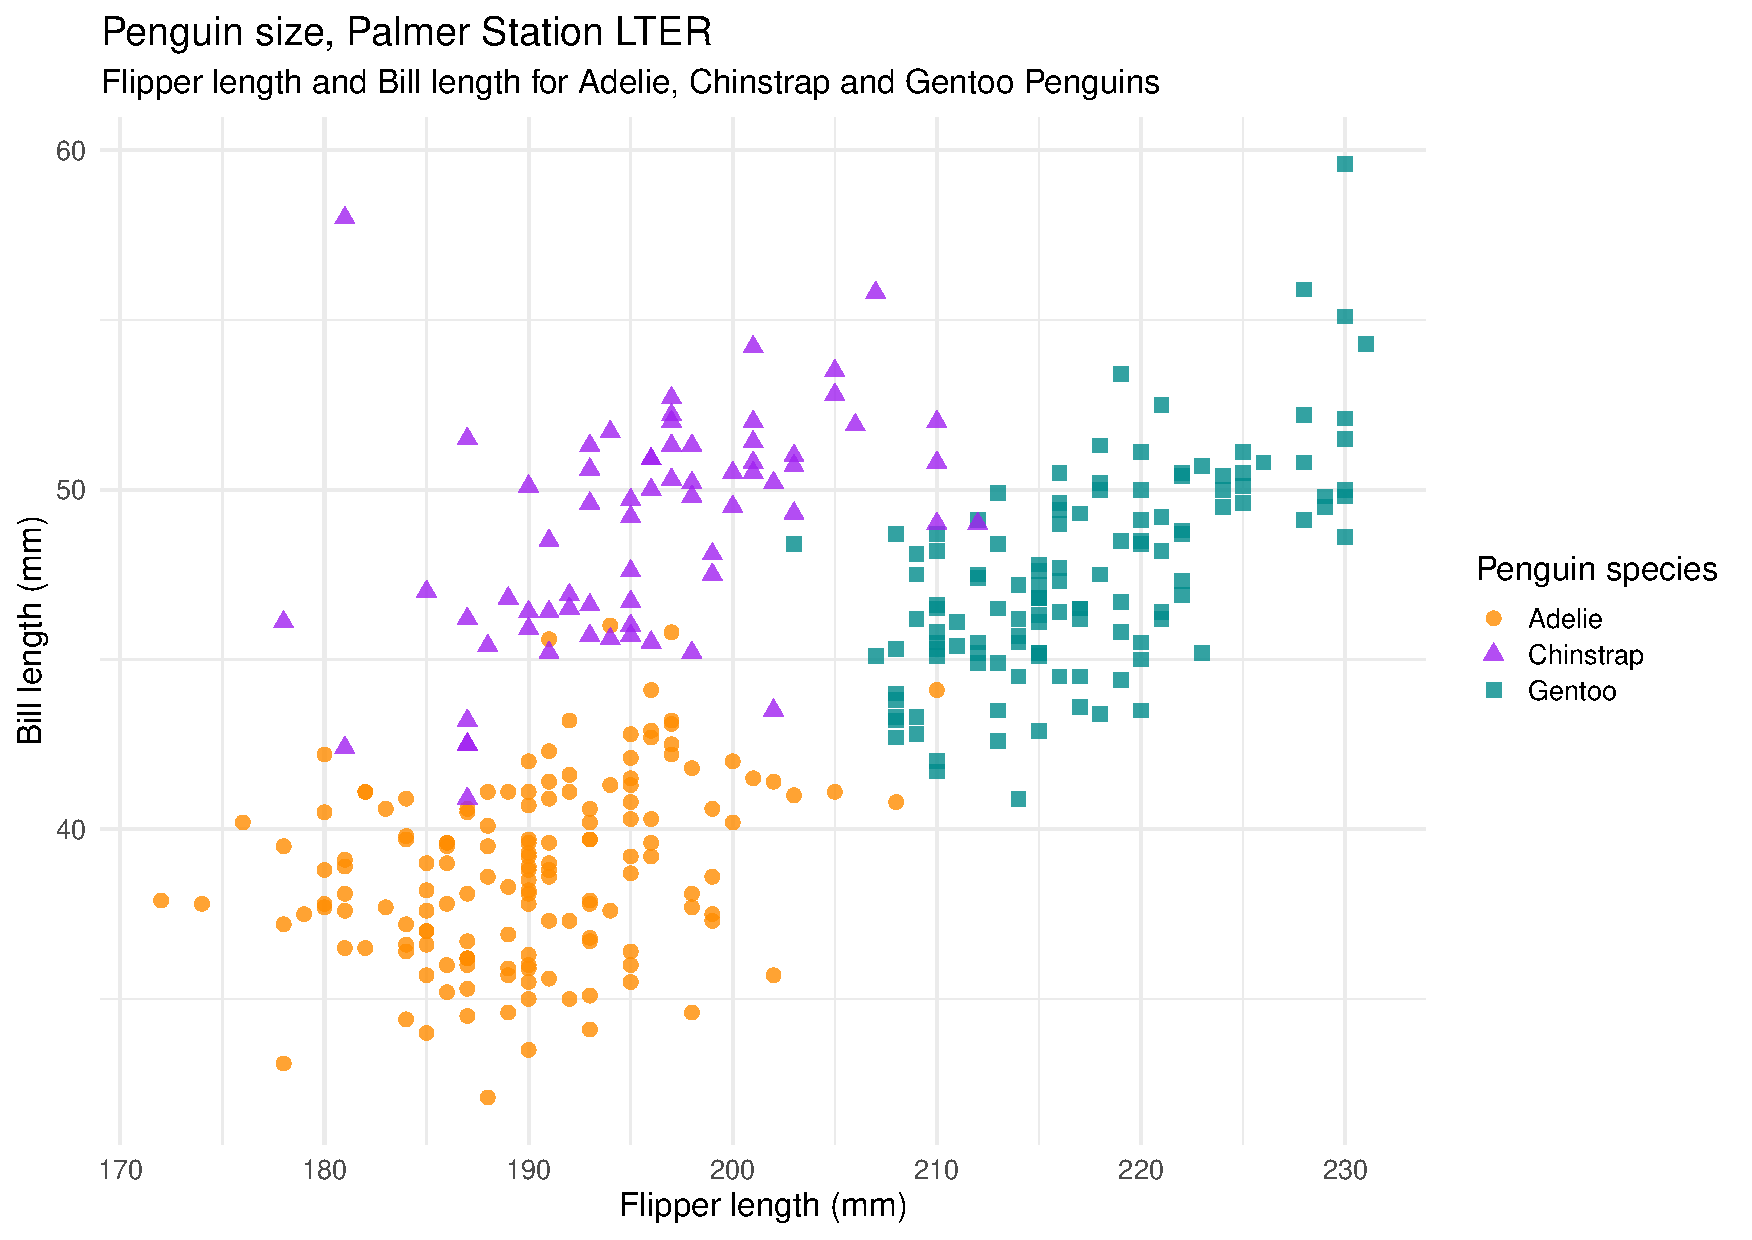
\includegraphics[width = 8cm]{presentation/plotpen.pdf}
        \caption{Plotting of Penguins Data}
        \label{fig:penplot}
    \end{figure}
\end{frame}

\begin{frame}{First Split}
    \begin{figure}
        \centering
        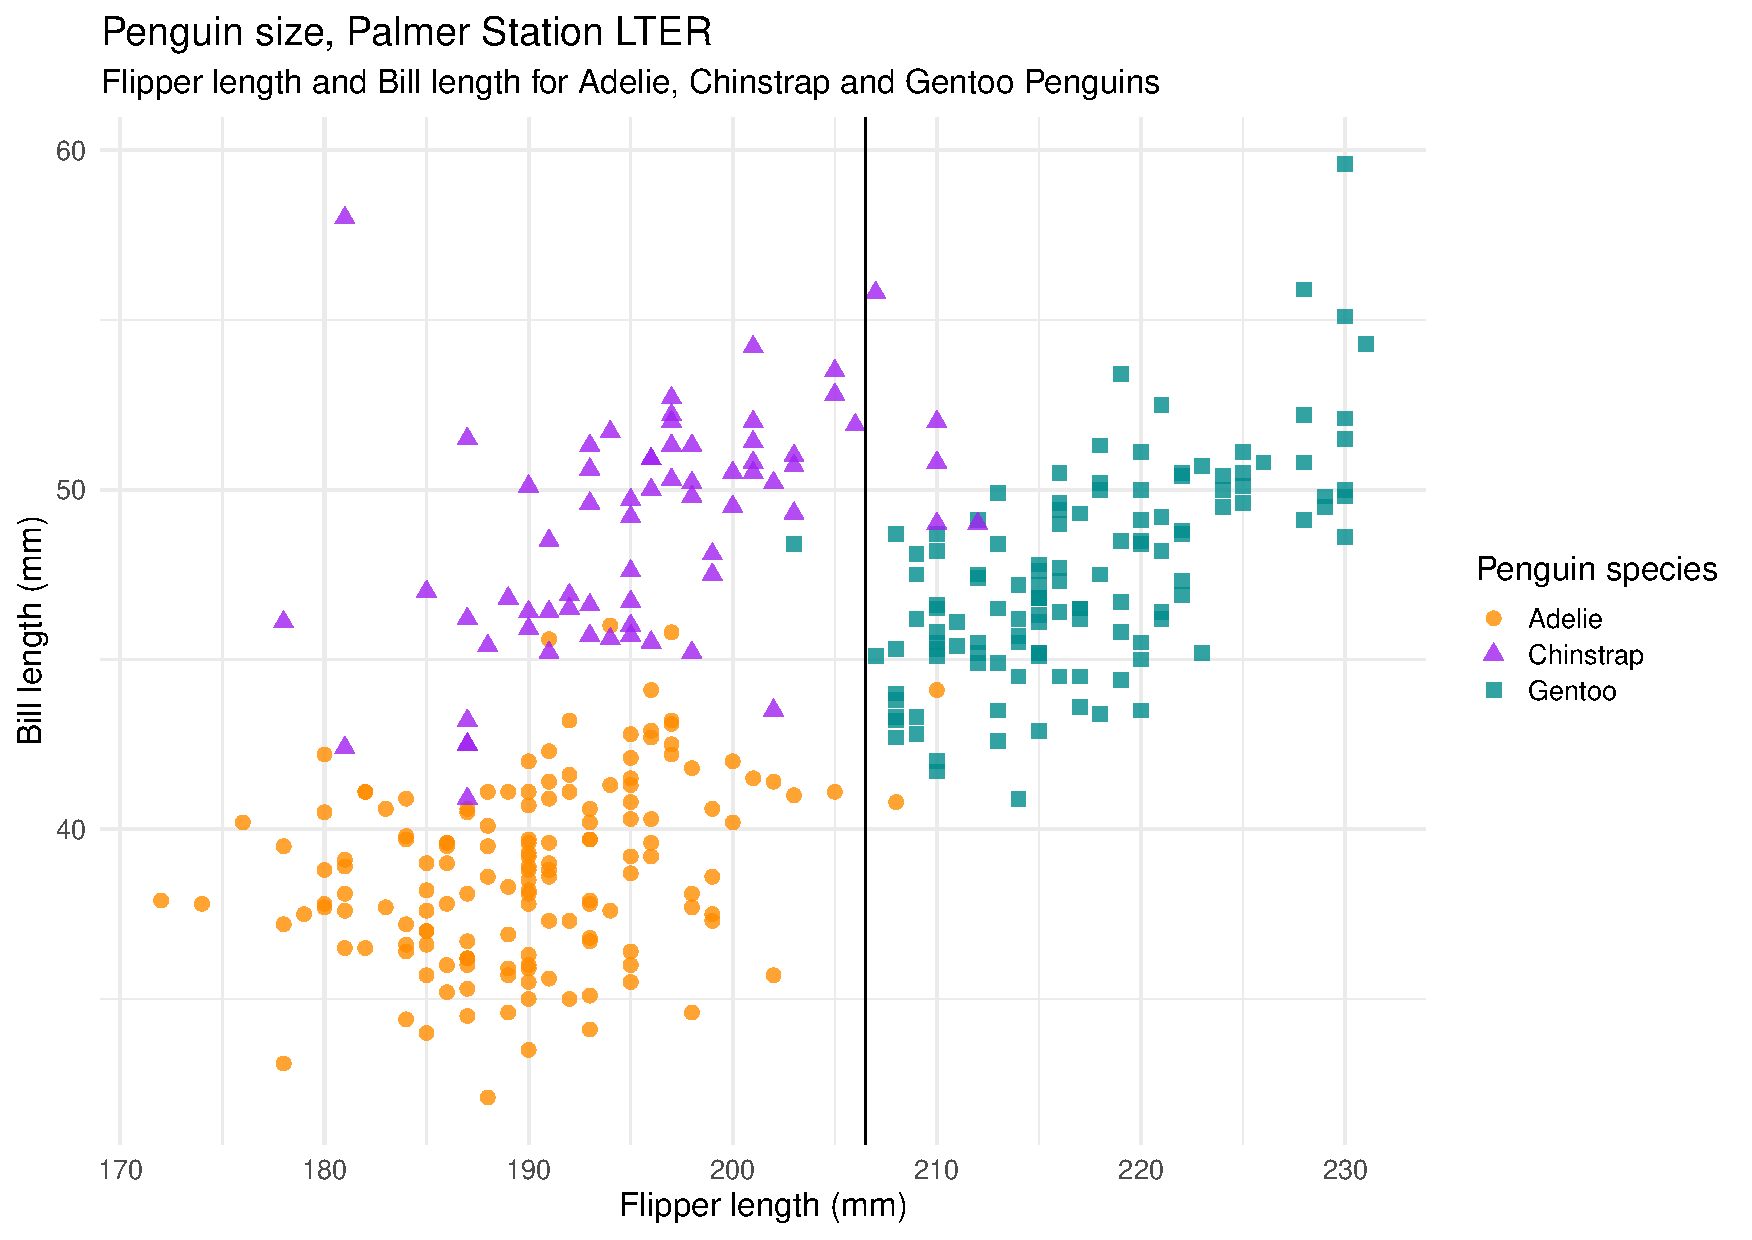
\includegraphics[width = 8cm]{presentation/plotpen1.pdf}
        \caption{x = 206.5}
        \label{fig:pen1}
    \end{figure}
\end{frame}

\begin{frame}{Second Split}
    \begin{figure}
        \centering
        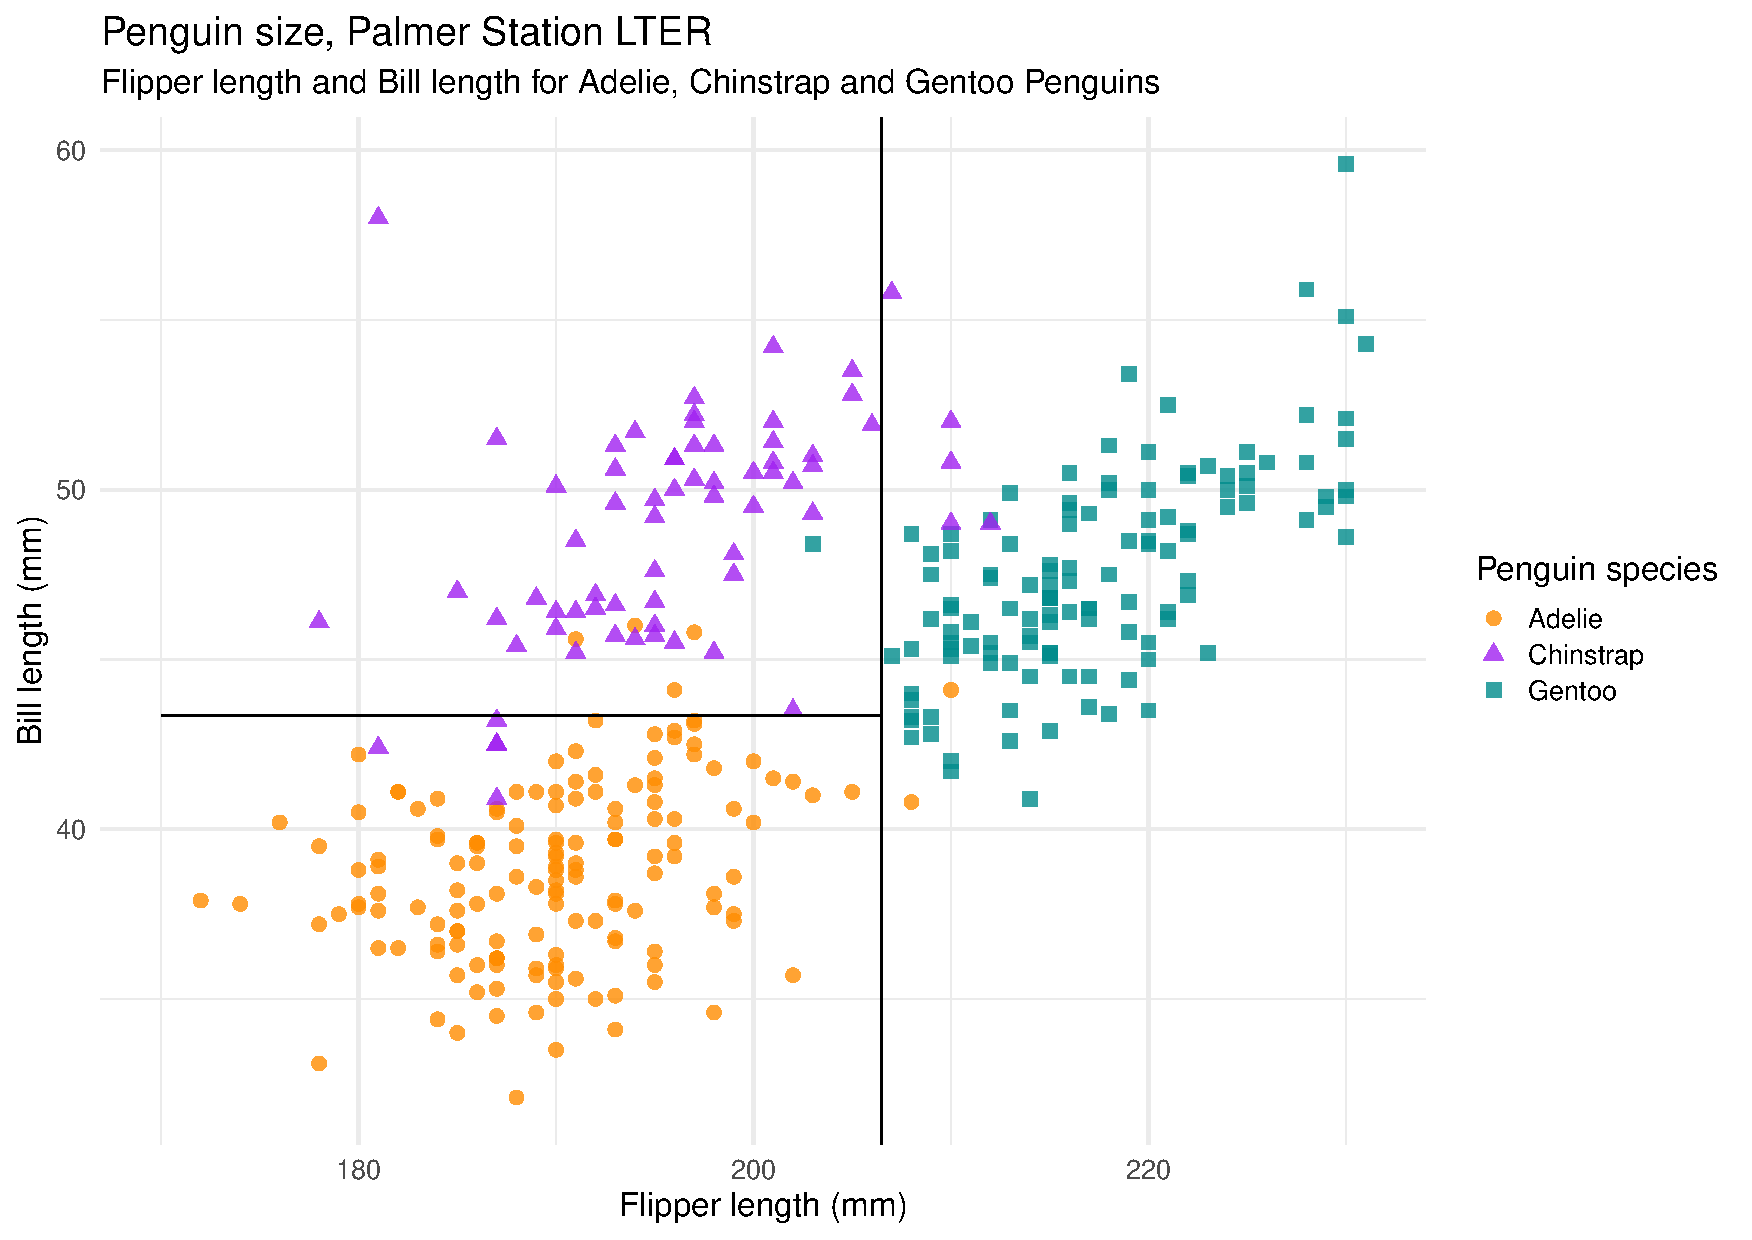
\includegraphics[width = 8cm]{presentation/plotpen2.pdf}
        \caption{On left split, y = 43.35}
        \label{fig:pen2}
    \end{figure}
\end{frame}

\begin{frame}{Regression Metrics}
    The residual sum squares is calculated as follows:
    \begin{equation}
    RSS = \sum_{m=1}^{M} \sum_{i \in R_m} (y_i - \hat{y}_{R_m})^2
 \end{equation}
 Where we have $m = 1,\dots,M$ regions and $\hat{y}_{R_m}$ is the predicted value of that region
\end{frame}

\begin{frame}{Classification Metrics}
CART uses Gini Impurity to calculate \textit{misclassification} of a parameter
\begin{equation}
    I_G (p) = I_G (p_1, \dots, p_M) = \sum_{i=1}^{M} p_i(1-p_i)
\end{equation}
With $m = 1,\dots,M$ classes and probabilities $p_i$ with $\sum_{i=1}^{M} p(i) = 1$.
\medskip\\
This chooses the variable with the highest impurity as the choice of split
\end{frame}

\begin{frame}{Information Gain}
    An alternative proposed by Quinlan \cite{Quinlan}
    \[  I_G(T,a) = -\sum_{i=1}^{n} p_i \log p_i 
    + \sum_{i=1}^{n} P(i \mid a) \log_2 P(i \mid a) \]
    With probabilities $p_i$, and $P(i \mid a)$ the proportion of the group that was split into one child node $a$ from the parent node.
    \medskip\\
    This chooses the split which results in us getting the largest increase in information by that split. 
\end{frame}

\begin{frame}{Algorithm to Growing Trees}
    \begin{enumerate}
     \item Use recursive splitting at all points into regions $R_1, R_2$ such that for a splitting value $s$, we have that for each value $x_i$, $i \in [1, \dots, n]$:
     \begin{enumerate}
         \item $R_1 = x_i \leq s$
         \item $R_2 = x_i > s$
     \end{enumerate}
     and classify each prediction in region based on the mean/modal value in each region
     
     \item Calculate the metric value for each region
     
     \item Compare metric values to find the most optimal splitting point
     
     \item Repeat until stopping criterion met
 \end{enumerate}
\end{frame}



\begin{frame}{Pruning}
    The idea of pruning is to minimise the cost-complexity criterion $C_{\alpha} (T)$:
    \begin{equation}
        C_{\alpha} (T) = R(T) + \alpha \left|T\right|
    \end{equation}
    Where $R(T)$ is the learning error, $\left|T\right|$ the number of terminal nodes in tree $T$, and $\alpha$ the regularization parameter. We find that $\alpha$ can be obtained from:
    \[ \alpha = \frac{R(t)-R(T_t)}{|T_t| - 1} \]
    And we are able to select the smallest value of $\alpha$ which minimizes $C_{\alpha} (T)$.
\end{frame}

\begin{frame}{Pruning Algorithm}
\begin{enumerate}

    \item Initialization - Let $T^1$ be the tree obtained with $\alpha^1 = 0$ by minimizing $R(T)$
    
    \item Select $t \in T^1$ which minimizes
        \[ g_1 (t) = \frac{R(t)-R(T_t^1)}{|T_t^1| - 1} \]
    
    \item Let $t_1$ be this node and let $\alpha^2 = g_1 (t_1)$ which results in $T^2 = T^1 - T_{t_1}^1$
    
    \item Repeat the process $i$ times until at cost $k$

\end{enumerate}
\end{frame}

\begin{frame}{Pima Data to Show Pruning}
Here, we will us the Pima Dataset from MASS \cite{MASS} to show how pruning allows us to grow better trees
\begin{figure}
    \centering
    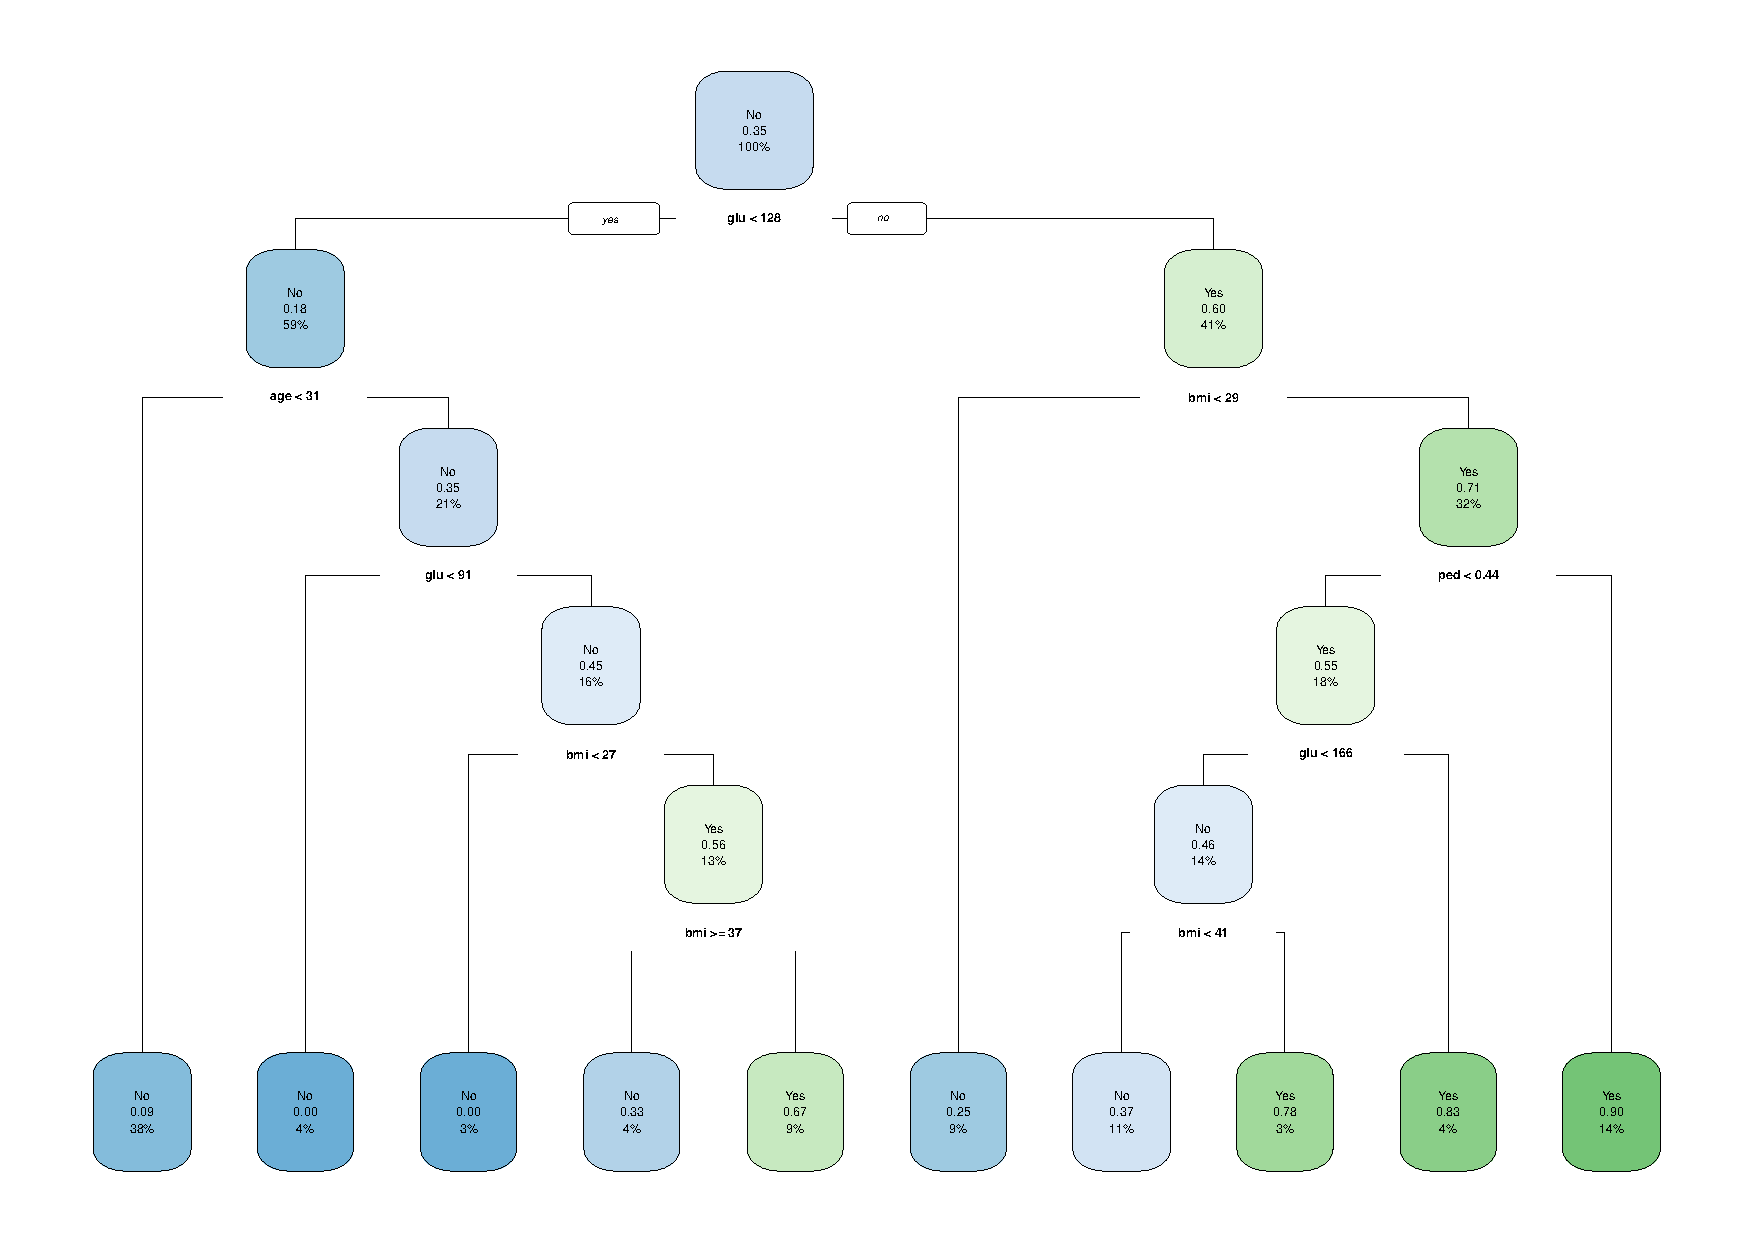
\includegraphics[width=7cm]{presentation/pimatrain.pdf}
    \caption{Full Pima Classification Tree}
    \label{fig:pima1}
\end{figure}
\end{frame}

\begin{frame}{Pruned Pima}
\begin{figure}
    \centering
    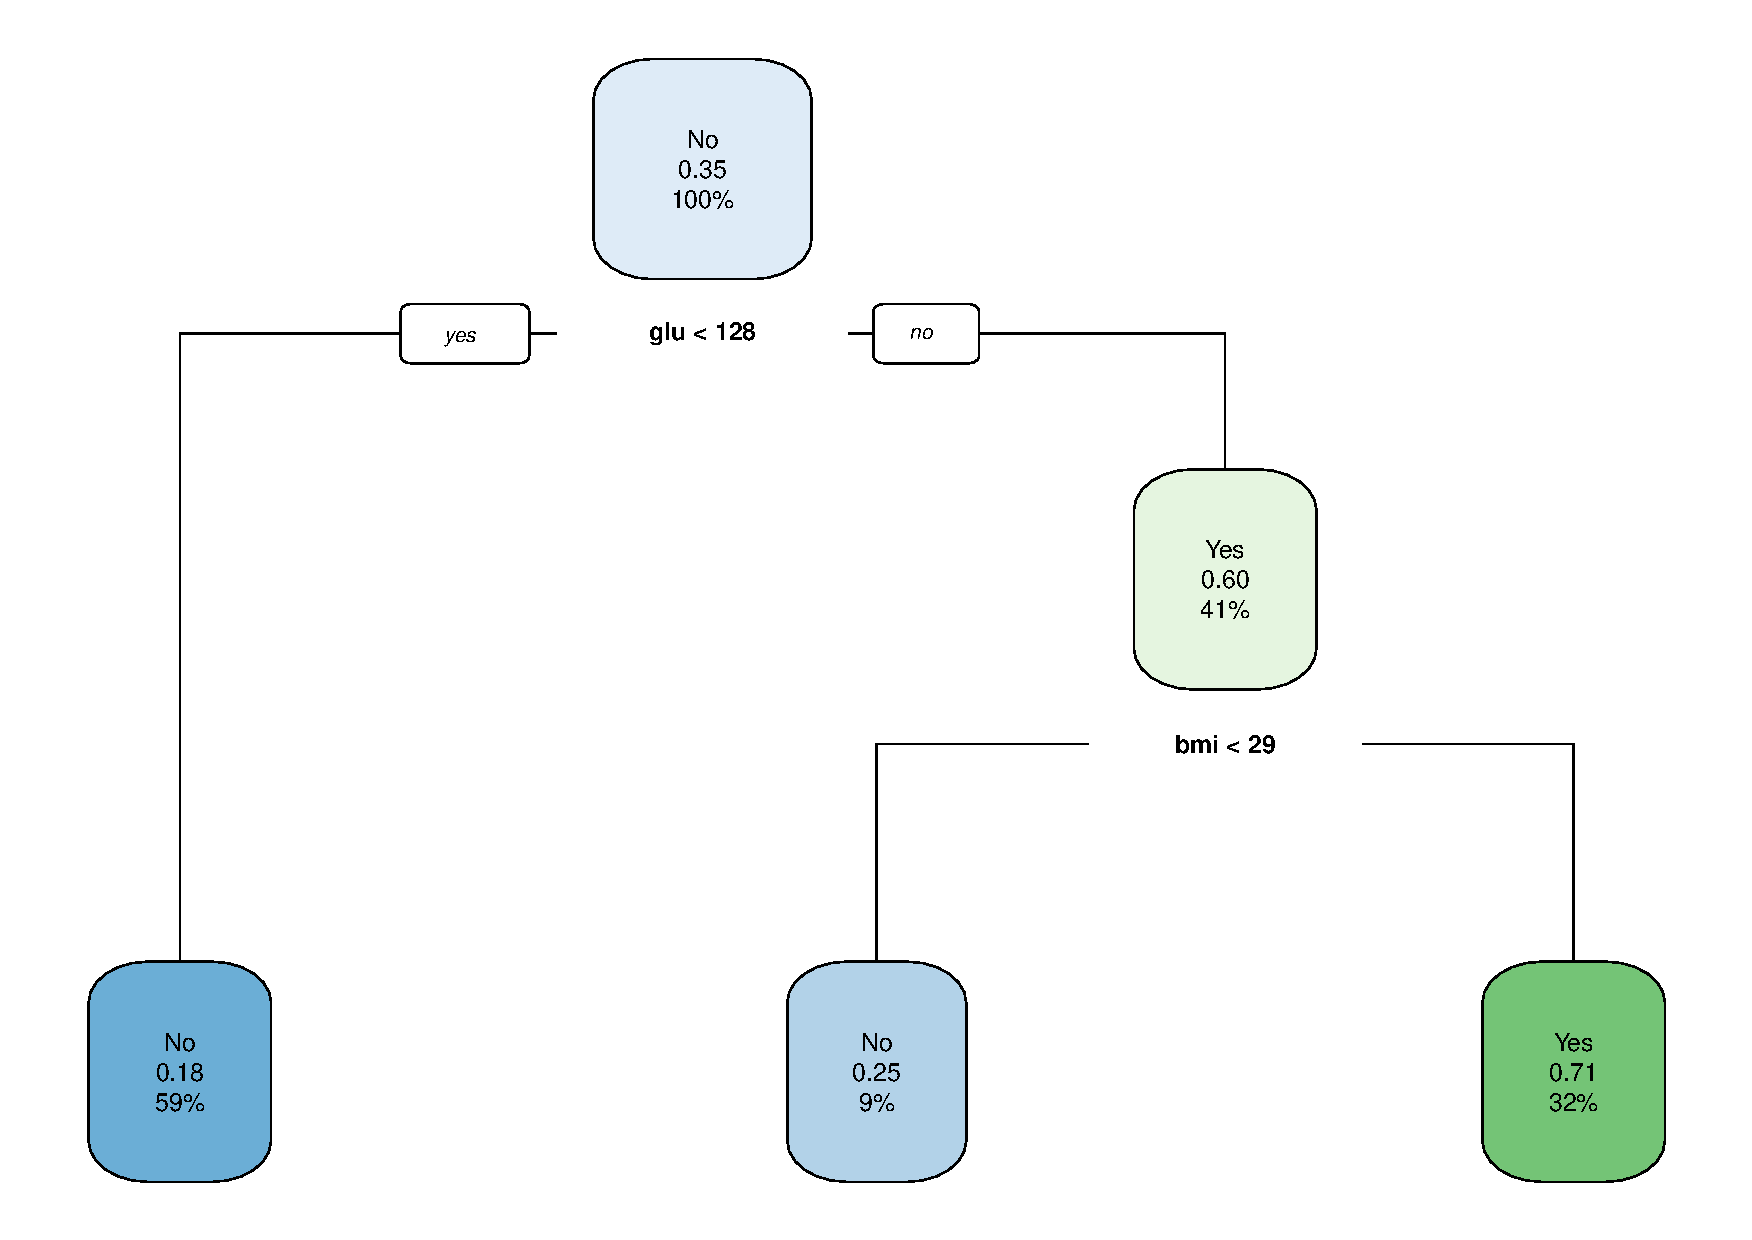
\includegraphics[width=7cm]{presentation/pimaprune.pdf}
    \caption{Pruned Pima Tree}
    \label{fig:pima2}
\end{figure}
\end{frame}

\begin{frame}{Comparison}
\begin{figure}
\centering
\begin{subfigure}{0.4\linewidth}
    \centering
    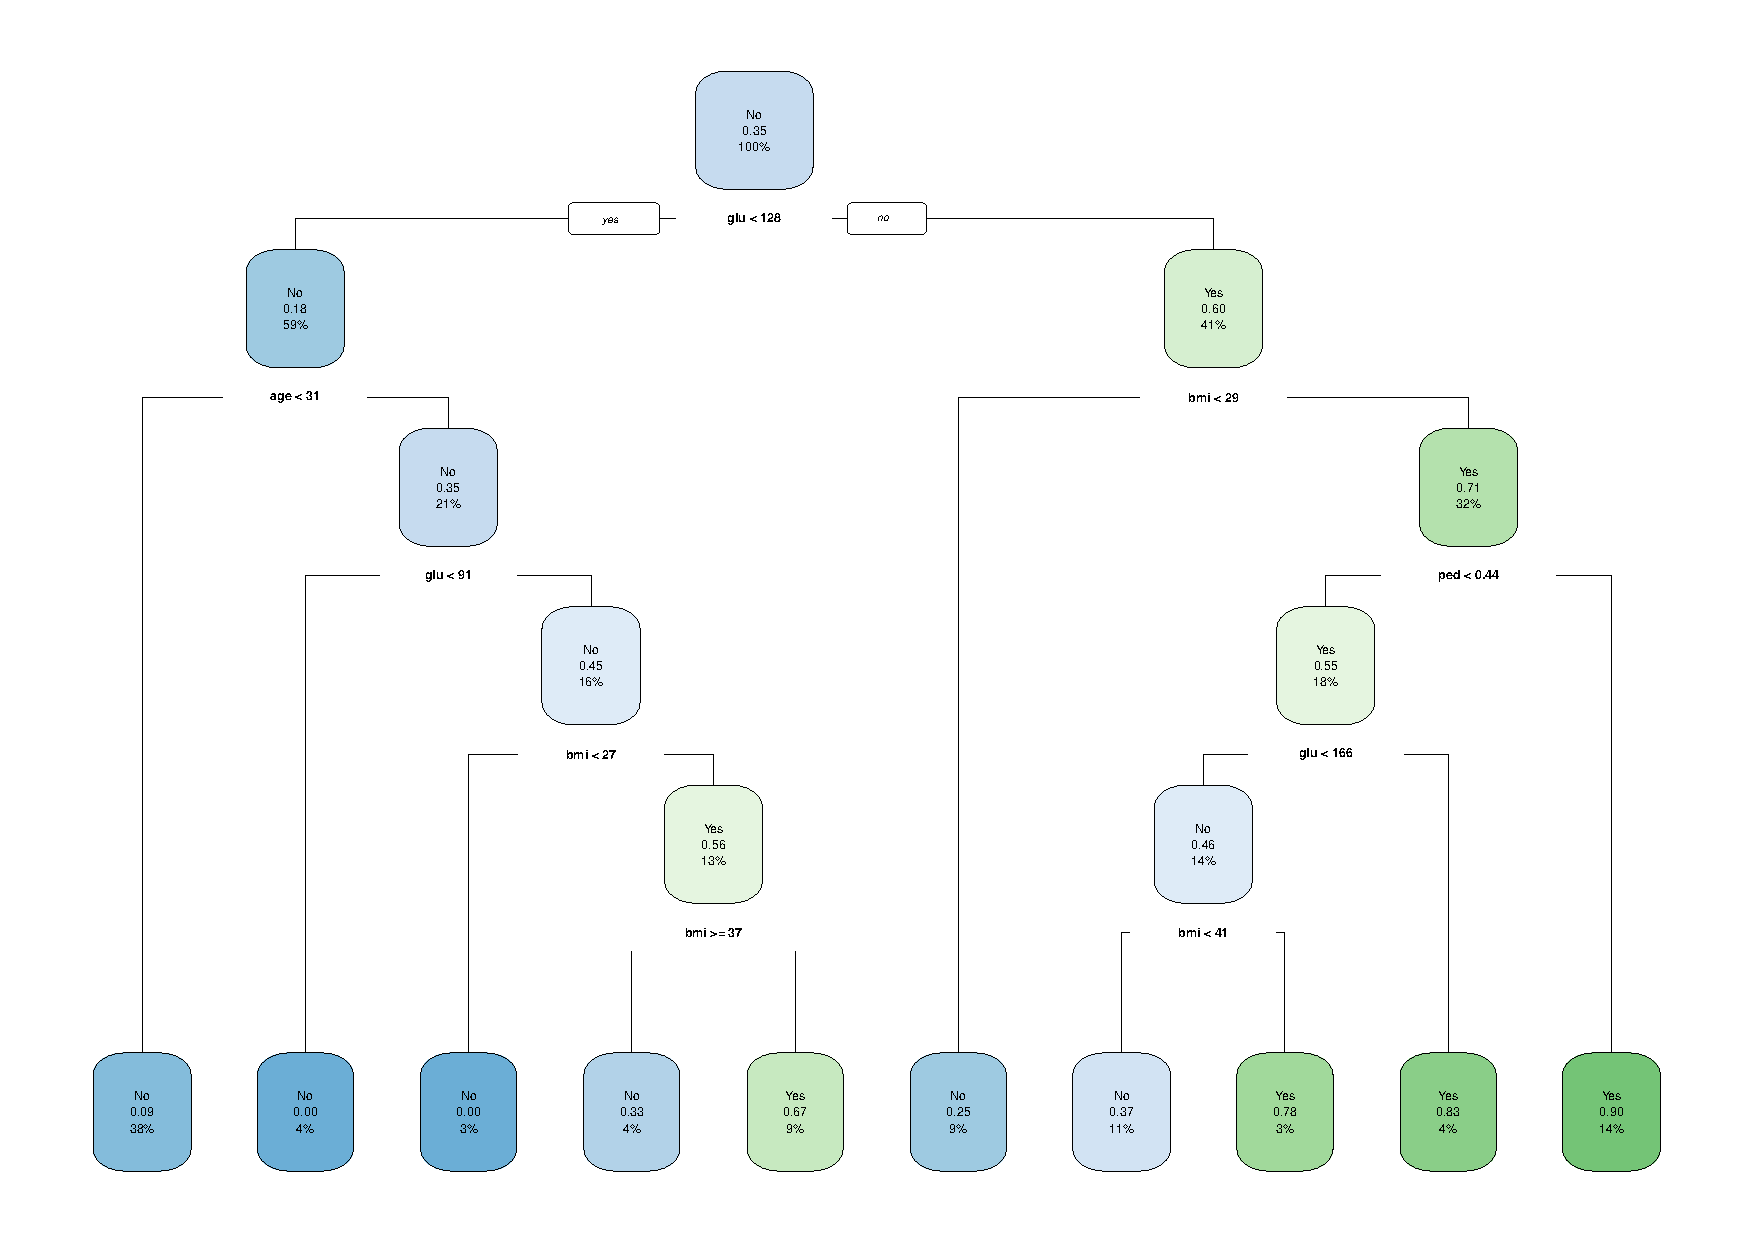
\includegraphics[width = 3.5cm]{presentation/pimatrain.pdf}
    \caption{Regular Pima Tree}
    \label{fig:pima3}
\end{subfigure}
\begin{subfigure}{0.4\linewidth}
    \centering
    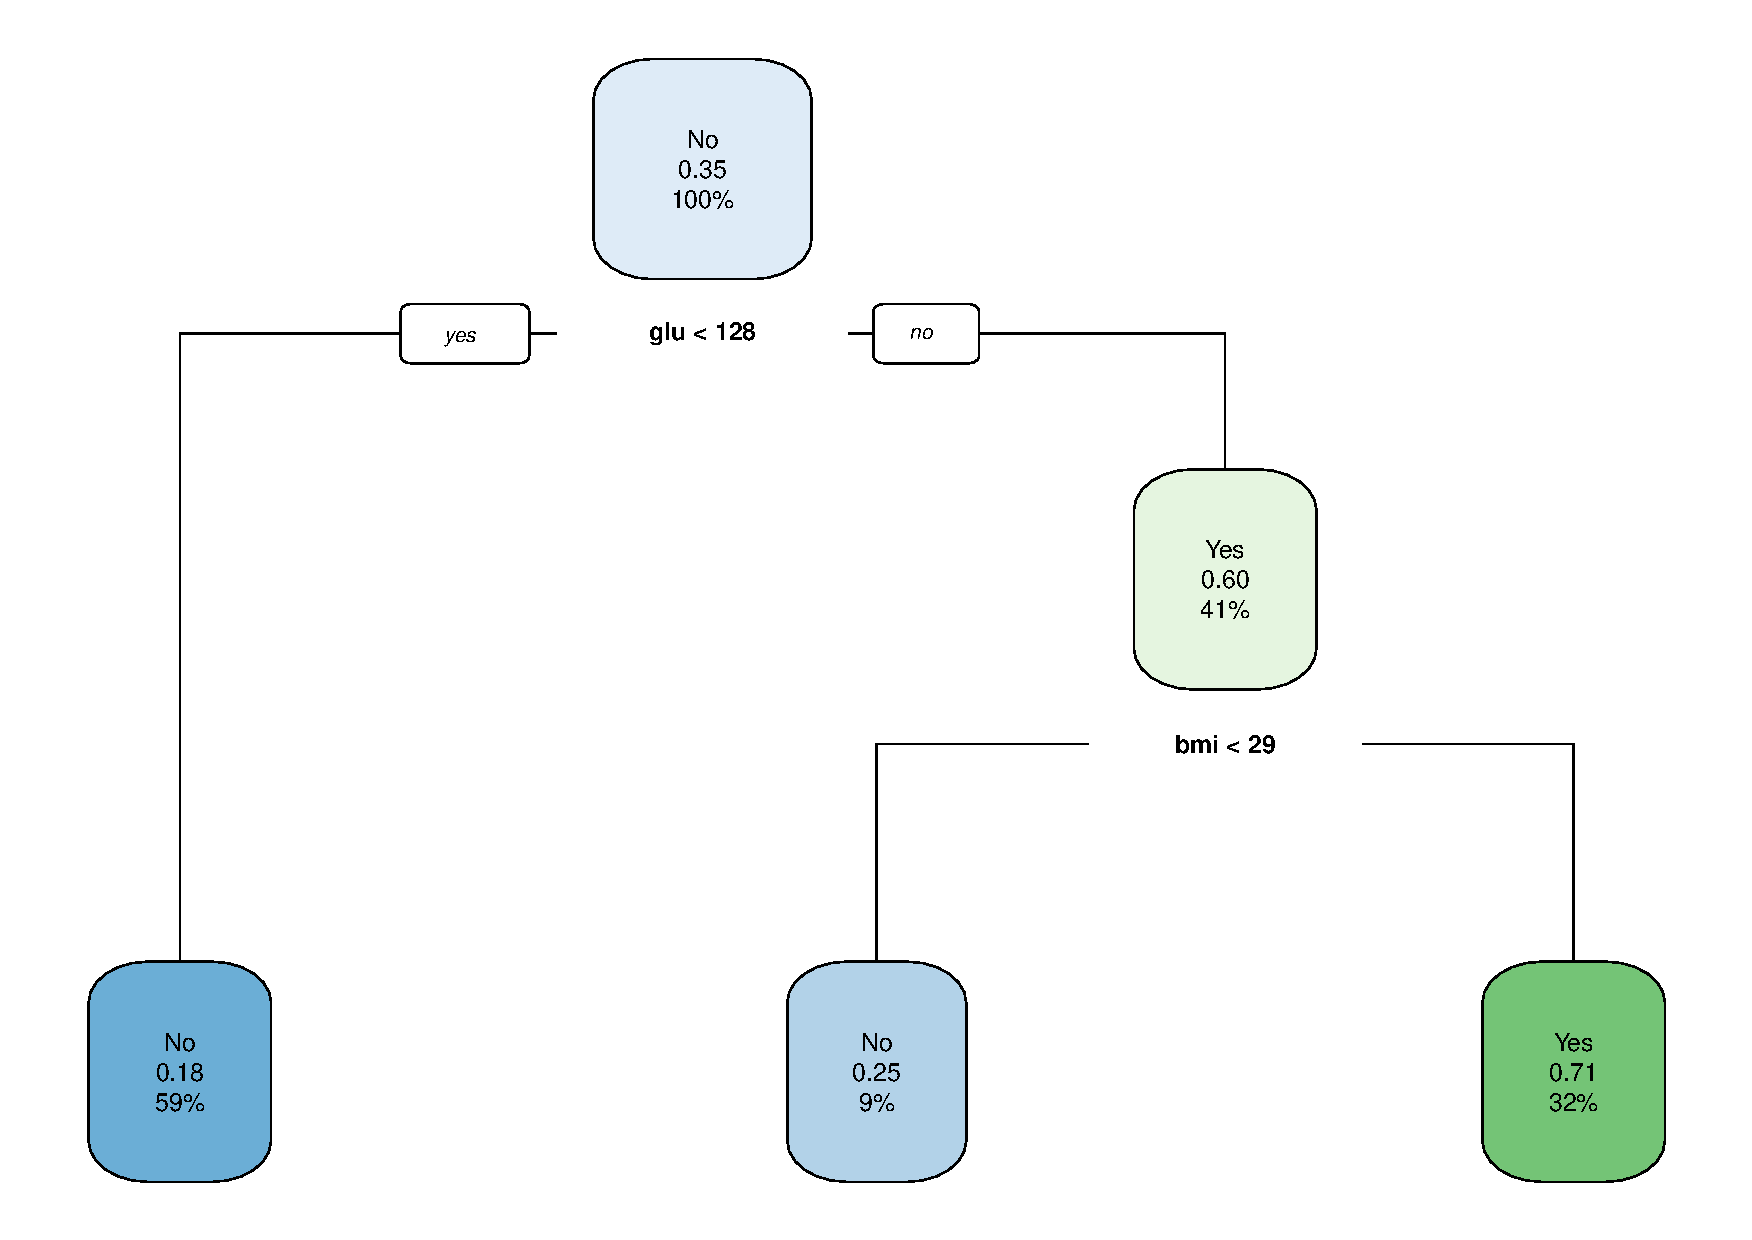
\includegraphics[width = 3.5cm]{presentation/pimaprune.pdf}
    \caption{Pruned Pima Tree}
    \label{fig:pima4}
\end{subfigure}
\caption{Comparision of Pima Data}
\label{fig:pima}
\end{figure}  
\end{frame}

\begin{frame}{ROC Performance}
   Here we show how pruning affects performance of the Decision Tree using the Receiver Operating Characteristic Curve to show how well a model predicts data
   \begin{figure}
       \centering
       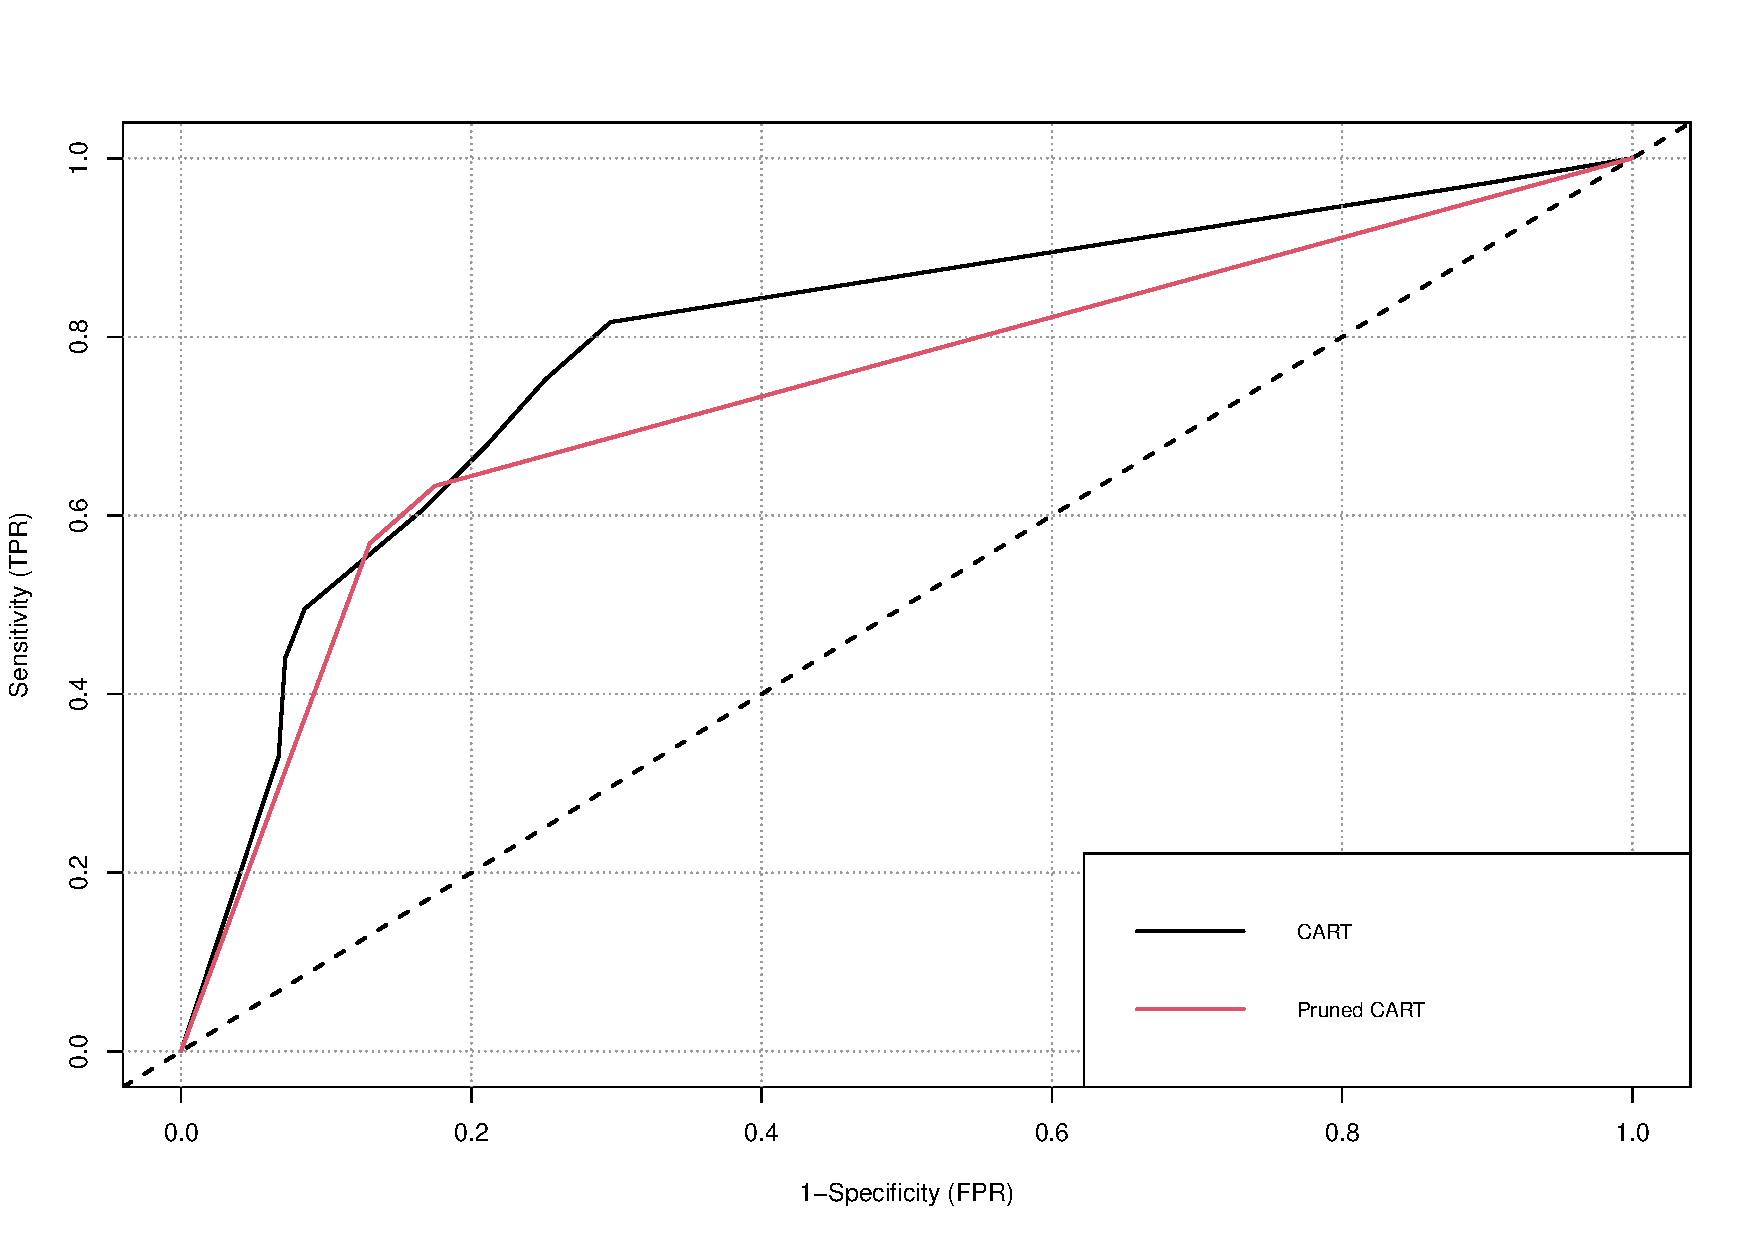
\includegraphics[width=6cm]{presentation/pimaroc.pdf}
       \caption{ROC Curve for the Pima Tree and the Pruned Tree}
       \label{fig:pimaroc}
   \end{figure}
\end{frame}

\begin{frame}{How to Improve Decision Trees}
    The \underline{heuristically greedy} nature of CART and other decision tree algorithms means that they tend to overfit data. 
    Many methods have been invented to try to solve this issue.
    \begin{itemize}
        \item<1-> \textbf{Bagging/Random Forests} - Invented by Leo Breiman \cite{randomforest}, they try to bootstrap multiple tree together to try to aggregate and minimize errors
        
        \item<2-> \textbf{Optimizing Decision Trees} - A new method (2017) \cite{oct} which aims to look at CART in the form of a Mixed-Integer Optimization Problem
    \end{itemize}
\end{frame}

\begin{frame}{A note on Optimized Decision Trees}
Optimized Decision Trees \cite{oct} uses a complexity parameter $\alpha$ controlling the tradeoff between accuracy and complexity, and a number in each node $N_{min}$ we aim to solve the problem $\forall \ l$ leaf nodes $ \in T$ tree:
\[ \begin{array}{cc}
        \min  & R(T) + \alpha \left|T\right|\\
        \text{s.t.}  & N(l) \geq N_{min}
    \end{array} \]
Where $N(l)$ is the number of points in leaf node $l$ and $R(T)$ is the misclassification error from before.
\end{frame}

\begin{frame}[allowframebreaks]
        \frametitle{References}
        \bibliographystyle{acm}
        \bibliography{reference}
\end{frame}


\end{document}